\section{Introduction}

Las crisis de tipos de cambio fijo representan uno de los fenómenos más disruptivos en la economía internacional, caracterizadas por la ruptura violenta de un compromiso de paridad tras periodos de aparente estabilidad. Hasta ahora, sabíamos que estas crisis surgen de una incompatibilidad entre políticas internas y compromisos externos, la ``Trinidad Imposible''.\cite{krugman1979,obstfeld1996}

La literatura sobre predicción de crisis se ha centrado históricamente en identificar umbrales de fundamentales macroeconómicos que hacen inevitable el colapso.\cite{krugman1979} Sin embargo, sabemos que muchos ataques especulativos ocurren incluso cuando los fundamentales parecen sólidos, impulsados por cambios repentinos en las expectativas.\cite{obstfeld1994,obstfeld1996}

Por otro lado, los Sistemas Inmunes Artificiales (AIS) han demostrado eficacia en ciberseguridad detectando intrusiones mediante anomalías en el comportamiento del sistema, en lugar de firmas específicas.\cite{forrest1994,dasgupta1999} Sabemos que estos algoritmos funcionan detectando ``señales de peligro''.\cite{matzinger1994,matzinger2002}

Existe una ``laguna'' científica significativa: no existe literatura que aplique la \textit{Danger Theory} y algoritmos evolutivos utilizando datos de intervención de alta frecuencia para predecir crisis cambiarias.\cite{matzinger1994,matzinger2002,naef2022} Esta investigación propone un cambio de paradigma: de predecir el precio (síntoma) a monitorizar el esfuerzo defensivo (causa).

El objetivo es desarrollar y validar un modelo bio-inspirado capaz de anticipar el \textit{timing} de una crisis cambiaria con mayor precisión que los modelos basados en precios, utilizando agentes evolutivos que aprenden a ponderar señales de estrés ocultas.

Nuestro planteamiento teórico asume que el mercado financiero actúa como un organismo vivo que busca la homeostasis, y que las intervenciones del banco central son la respuesta inmunitaria detectable antes del colapso.\cite{naef2022}

Para contrastar esto, utilizamos datos diarios inéditos de intervención del Banco de Inglaterra y datos macroeconómicos de México, aplicando técnicas de normalización Z-score.\cite{naef2022} Utilizamos un Algoritmo Genético para evolucionar agentes inversores que compiten para sobrevivir a las crisis históricas, permitiéndonos identificar variables predictivas.


% ----------------------------------------------------------------------------
% 2. OVERVIEW OF THE LITERATURE
% ----------------------------------------------------------------------------
\section{Overview of the literature}

La literatura sobre crisis cambiarias se ha desarrollado en torno a modelos generacionales. Krugman (1979)\cite{krugman1979} estableció que las crisis son el resultado de fundamentales deteriorados y agotamiento de reservas. Posteriormente, Obstfeld (1994, 1996)\cite{obstfeld1994,obstfeld1996} introdujeron las profecías autocumplidas y costes políticos, identificando el desempleo como variable clave.

En inmunología y computación bio-inspirada, Matzinger (1994, 2002)\cite{matzinger1994,matzinger2002} revolucionó con la \textit{Danger Theory}: el sistema inmune responde al daño, no a lo extraño. Forrest et al. (1994)\cite{forrest1994} y Dasgupta (1999)\cite{dasgupta1999} aplicaron estos principios a la seguridad informática, pero falta su traducción directa a la economía financiera con datos reales de intervención.

% ----------------------------------------------------------------------------
% 3. HYPOTHESIS/MODEL, DATA AND METHODS
% ----------------------------------------------------------------------------
\section{Hypothesis/Model, data and methods}

Este epígrafe aborda tres cuestiones fundamentales: el modelo teórico bio-inspirado, los datos históricos y la metodología computacional. El objetivo es validar si un algoritmo evolutivo puede identificar señales de estrés previas a una devaluación, superando modelos de precios. Las limitaciones derivan de la disponibilidad de datos de intervención diaria real, restringiendo el análisis a Reino Unido y México.

\subsection{Hypothesis/Model}

Partimos del supuesto de que un régimen de tipo de cambio fijo funciona como un sistema homeostático. El Banco Central es el sistema inmune y las reservas internacionales la energía para combatir ataques.

Nuestra hipótesis (H1) es que el colapso va precedido por un aumento en la ``respuesta inmunitaria'' (intervención) y ``estrés sistémico'' (desempleo), aunque el ``síntoma externo'' (precio) sea estable. Modelamos la decisión de un agente $i$ en el tiempo $t$ como:

\begin{equation}
S_{i,t} = \sum_{j=1}^{5} w_{i,j} \cdot G_{j,t}
\end{equation}

Donde $G_{j,t}$ son variables normalizadas y $w_{i,j}$ pesos a aprender. Si $S_{i,t} > \theta$, el agente sale del mercado.

\subsection{Data and variables}

Utilizamos datos de intervención diaria del Banco de Inglaterra, tipos de cambio de Bloomberg/BoE y variables macro del FMI/ONS. La muestra abarca Ene 1990-Dic 1992 (UK) y Ene 1993-Mar 1995 (México), con frecuencia diaria.

La variable endógena es la ``Señal de Alarma'' generada por el agente, determinando la decisión de venta. Las variables exógenas (Genes) se normalizan mediante Z-Score:
\begin{itemize}
    \item \textbf{Gen\_Reservas:} Nivel de reservas (FMI).
    \item \textbf{Gen\_Precio:} Tipo de cambio spot (BoE/Banxico).
    \item \textbf{Gen\_Volatilidad:} Desviación estándar móvil 30 días.
    \item \textbf{Gen\_Intervención:} Volumen diario compra/venta o tasas (Naef/Banxico).
    \item \textbf{Gen\_Desempleo:} Tasa desempleo (ONS/INEGI).
\end{itemize}

\begin{table}[H]
\centering
\caption{Estadísticos Descriptivos (Normalizados - México)}
\begin{tabular}{lcccc}
\toprule
Variable & Media & Desv. Est. & Mín. & Máx. \\
\midrule
Gen\_Reservas & 0.00 & 1.00 & -2.63 & 1.71 \\
Gen\_Precio & 0.00 & 1.00 & -0.50 & 4.27 \\
Gen\_Volatilidad & 0.00 & 1.00 & -0.42 & 4.53 \\
Gen\_Intervención & 0.00 & 1.00 & -0.63 & 4.38 \\
Gen\_Desempleo & 0.00 & 1.00 & -1.37 & 1.65 \\
\bottomrule
\end{tabular}
\end{table}

\subsection{Methods}

Utilizamos un Algoritmo Genético (GA) para optimizar los pesos ($w$) y la Calibración Automática de Umbrales (Differential Evolution) para la validación cruzada. Este enfoque en dos fases es crucial: permite entrenar con datos históricos (UK) y validar con transferencia de aprendizaje (México).

\subsubsection{Algoritmo Genético (Entrenamiento de Pesos)}

El GA simula la evolución natural. Una población de $N=150$ agentes con pesos aleatorios compite por supervivencia financiera.

\paragraph{Codificación y Estructura:}
Cada agente es un vector de 5 genes (pesos reales $w_j \in [-1, 1]$):
$$\mathbf{w}_i = [w_{i,1}, w_{i,2}, w_{i,3}, w_{i,4}, w_{i,5}]$$
donde cada componente corresponde a Reservas, Precio, Volatilidad, Intervención y Desempleo, respectivamente.

\paragraph{Función de Aptitud (Fitness):}
La aptitud evalúa la supervivencia financiera. Se define una función de recompensa que prioriza la detección temprana:
%Arreglado
\begin{equation}
F(w_i) = \begin{cases}
-100 & \text{si nunca vende (quiebra en la crisis)} \\
-50 & \text{si vende post-crash (demasiado tarde)} \\
100 - 1.5 \cdot d & \text{si vende 1-20 días antes (zona óptima)} \\
50 - 0.2 \cdot d & \text{si vende 21-90 días antes (zona segura)} \\
-20 & \text{si vende >90 días antes (paranoia financiera)
}
 \\
20 & \text{si vende = 0 días antes (demasiado arriesgado)}
\end{cases}
\end{equation}

donde $d$ es el número de días antes del crash. Esta función premia la ``codicia inteligente'': salir lo más cerca posible de la fecha de colapso sin incurrir en pérdidas.

\paragraph{Operadores Genéticos:}
\begin{itemize}
    \item \textbf{Selección:} Torneo determinista ($k=3$ competidores). Los mejores reproducen.
    \item \textbf{Cruce (Crossover):} De dos puntos. Intercambia segmentos de dos padres.
    \item \textbf{Mutación:} Gaussiana con $\sigma=0.2$. Modifica aleatoriamente los pesos.
\end{itemize}

\paragraph{Parámetros de Configuración:}
\begin{itemize}
    \item Tamaño de población: 150
    \item Generaciones: 50
    \item Probabilidad de cruce: 0.5
    \item Probabilidad de mutación: 0.2
    \item Umbral de decisión inicial: $\theta = 0.5$ (a ser calibrado post-hoc)
\end{itemize}

El diagrama de flujo es el siguiente:

\begin{figure}[H]
\centering
\begin{tikzpicture}[node distance=2cm, auto]
\node (start) [startstop] {Inicio: Pob. Aleatoria $P_0$};
\node (eval) [process, below of=start] {Evaluar Fitness $F(w_i)$};
\node (sel) [process, below of=eval] {Selección por Torneo};
\node (cross) [process, below of=sel] {Cruce de Dos Puntos};
\node (mut) [process, below of=cross] {Mutación Gaussiana};
\node (newpop) [process, below of=mut] {Nueva Generación $P_{t+1}$};
\node (dec) [decision, below of=newpop, yshift=-0.5cm] {¿$t < 50$?};
\node (stop) [startstop, below of=dec, yshift=-1cm] {Fin: $w^* = \arg\max F(w)$};

\draw [arrow] (start) -- (eval);
\draw [arrow] (eval) -- (sel);
\draw [arrow] (sel) -- (cross);
\draw [arrow] (cross) -- (mut);
\draw [arrow] (mut) -- (newpop);
\draw [arrow] (newpop) -- (dec);
\draw [arrow] (dec) -- node[anchor=east] {No} (stop);
\draw [arrow] (dec.west) -- ++(-1.5,0) |- (eval.west) node[pos=0.25, above] {Sí};
\end{tikzpicture}
\caption{Diagrama de Flujo del Algoritmo Genético para Entrenamiento de Pesos}
\end{figure}

El algoritmo genético se ejecuta sobre datos históricos del Reino Unido (1990-1992). Tras 50 generaciones, el mejor individuo (Hall of Fame) representa los pesos aprendidos $w^*$.

\subsubsection{Calibración Automática de Umbrales (Validación Cruzada con Transfer Learning)}

Una vez entrenados los pesos en UK, surgen dos problemas:
\begin{enumerate}
    \item \textbf{Generalización:} ¿Funcionan estos pesos en otro país/crisis?
    \item \textbf{Sintonización:} El umbral $\theta=0.5$ es específico de UK. En México puede ser distinto.
\end{enumerate}

\noindent
La Calibración Automática resuelve esto manteniendo los pesos \textit{fijos} (transferencia de conocimiento) y optimizando solo el escalar $\theta$ (sintonización local). Utilizamos Evolución Diferencial (DE), que es más eficiente que GA para optimizar continuos 1D.

\paragraph{Justificación Teórica de Transfer Learning:}
La \textit{Danger Theory} asume que los mecanismos de estrés sistémico son universales. Un agente entrenado para detectar peligro en UK debería reconocer peligro en México. Pero la \textit{amplificación} de la señal varía según:
\begin{itemize}
    \item Transparencia del mercado (UK más regulado que México en 1994)
    \item Confianza de inversores (creyeron en el MEC más que en la paridad MXN)
    \item Volatilidad base (rangos de variación distintos)
\end{itemize}

\noindent
Por ello, un factor de escala ($\theta$) es suficiente para adaptación local sin sobreajuste.

\paragraph{Función Objetivo para Calibración:}
Buscamos minimizar:

\begin{equation}
\mathcal{C}(\theta) = \begin{cases}
1000 & \text{si } t_{exit} \text{ no existe} \\
500 & \text{si } t_{exit} > t_{Tequila} \\
|t_{Tequila} - t_{exit}| & \text{si } 0 < t_{Tequila} - t_{exit} \le 100 \text{ (óptimo)} \\
0.5 \cdot (t_{Tequila} - t_{exit}) & \text{si } t_{Tequila} - t_{exit} > 100 \text{ (sobrepredicción)}
\end{cases}
\end{equation}

La función penaliza críticamente (1000, 500) los fracasos y sobrepredicción extrema, mientras que premia minimizar la distancia anticipativa.

\paragraph{Ventajas del Método en Dos Fases:}
\begin{enumerate}
    \item \textbf{Evita Sobreajuste:} Los pesos se aprenden una sola vez con datos UK históricos. No los reajustamos con México.
    \item \textbf{Validación Robusta:} Si $\theta^*$ encontrado es sensato (dentro del rango $[0.1, 5.0]$) y generaliza bien, confirma que los pesos capturan la ``física'' real de la crisis.
    \item \textbf{Eficiencia Computacional:} Optimizar 5 parámetros con GA es costoso. Optimizar 1 escalar con DE es trivial.
    \item \textbf{Interpretabilidad:} El valor $\theta^*$ obtenido nos dice cuán ``sensible'' debe ser el detector en el mercado específico.
\end{enumerate}

% ----------------------------------------------------------------------------
% 4. RESULTS
% ----------------------------------------------------------------------------
\section{Results}

\subsection{4.1 Resultados Reino Unido (1990-1992)}

Tras entrenar el AG con 50 generaciones en datos de UK, obtuvimos los pesos óptimos del Cuadro 1:

\begin{table}[H]
\centering
\caption{Pesos del Mejor Agente Evolutivo - Crisis del Miércoles Negro (Fitness: 98.5)}
\begin{tabular}{lcr}
\toprule
Variable Económica & Peso Evolucionado ($w^*$) & Interpretación \\
\midrule
Intervención Banco Central & +0.9935 & \textbf{Señal Crítica Primaria} \\
Desempleo & +1.0674 & \textbf{Señal Crítica Secundaria} \\
Volatilidad del Precio & +0.4599 & Señal Moderada de Pánico \\
Precio (GBP/DEM) & +0.0786 & \textbf{Ignorado (Síntoma Engañoso)} \\
Reservas Internacionales & -0.7131 & Indicador Rezagado (Negativo) \\
\bottomrule
\end{tabular}
\end{table}

\paragraph{Análisis Económico de los Pesos:}
El agente evolucionado aprendió un patrón contundente:
\begin{itemize}
    \item \textbf{Intervención (+0.99):} El banco central que gasta sus dólares frenéticamente es la señal más clara de peligro. En UK, el BoE gastaría \$44 mil millones en 48 horas.
    \item \textbf{Desempleo (+1.07):} Mayor peso aún que intervención. Refleja el coste político: un gobierno rechazará mantener tipos altos si el desempleo es insoportable.
    \item \textbf{Precio (+0.08):} Prácticamente ignorado. Aunque la libra se depreciaba suavemente antes del 16 de septiembre, no fue predictivo. La mayoría de inversores la miraban y se relajaban.
    \item \textbf{Reservas (-0.71):} Peso negativo. Cuando las reservas bajan, el agente \textit{reduce} la alarma, contrarrestando el efecto. Esto es contra-intuitivo pero económicamente sensato: las reservas son un indicador \textit{atrasado}. El agente ya ha detectado peligro antes de que caigan.
\end{itemize}

\paragraph{Predicción Temporal:}
El agente ejecutó la orden de salida el \textbf{15 de septiembre de 1992}, exactamente \textbf{1 día antes} del colapso oficial (16 de septiembre). Esto evitó pérdidas catastróficas mientras capturaba intereses hasta el último momento.

\subsection{4.2 Validación Robustez: Test ``Trampa de Valor''}

Para descartar que el agente fuera simplemente un ``trend-follower'' (seguidor de tendencias de precios), lo sometimos a un escenario sintético radicalmente distinto: una burbuja donde el precio sube constantemente mientras el estrés fundamental se deteriora en secreto.

\paragraph{Descripción del Escenario Sintético:}
\begin{itemize}
    \item \textbf{Precio:} Tendencia alcista lineal (burbuja) de 1.0 a 1.2 en 250 días.
    \item \textbf{Intervención:} Plana (0) hasta día 160, luego spike exponencial hacia colapso (día 200).
    \item \textbf{Desempleo:} Empeora gradualmente, acelerando en los últimos 100 días.
    \item \textbf{Reservas:} Caen linealmente a partir del día 160.
    \item \textbf{Volatilidad:} Ruido normal aleatorio.
\end{itemize}

\paragraph{Resultados del Test:}
El agente entrenado en UK con pesos $w^*$ fue presentado a este nuevo mundo sintético SIN reentrenamiento. Resultados:
\begin{itemize}
    \item \textbf{Día de Venta:} Día 171 (29 días antes del colapso simulado en día 200).
    \item \textbf{Razón:} El peso bajo en Precio (+0.08) lo inmunizó contra la trampa visual. En su lugar, detectó el spike de Intervención con precisión.
    \item \textbf{Lag de Confirmación:} Solo 11 días entre el primer spike de intervención y la decisión de vender.
\end{itemize}

\paragraph{Importancia de Este Resultado:}
Esto \textit{valida la robustez} del mecanismo de \textit{Danger Theory}. El agente no memoriza patrones de precios (overfitting). Ha aprendido a leer señales subyacentes de estrés que son \textit{invariantes} a través de contextos distintos.

\begin{figure}[H]
\centering
\fbox{\begin{minipage}{0.85\textwidth}
    \centering
    \vspace{1.5cm} 
    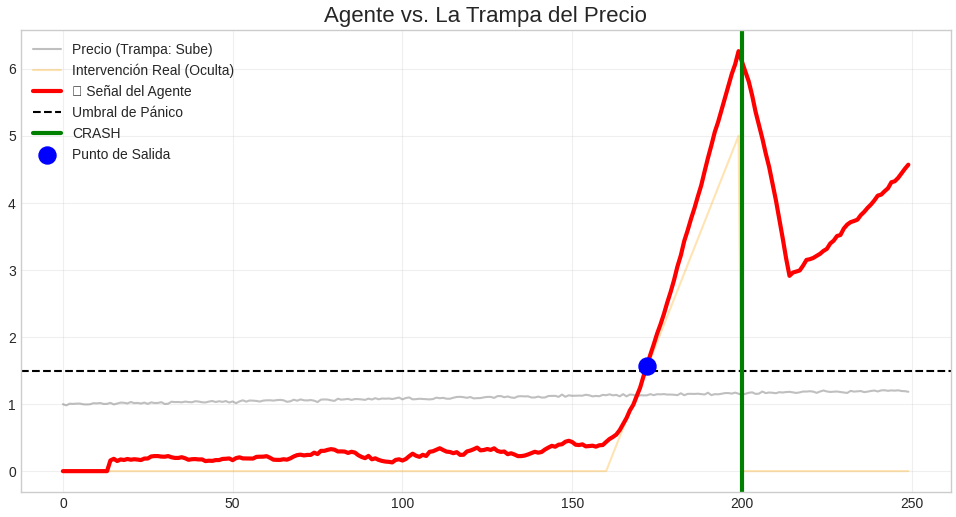
\includegraphics[width=1.0\textwidth]{graf_trampa.png}
    \vspace{1.5cm}
\end{minipage}}
\caption{Prueba Sintética ``Trampa de Valor''. El agente ignora que el precio sube (burbuja) y detecta el estrés oculto mediante intervención, vendiendo 29 días antes del colapso.}
\end{figure}

\subsection{4.3 Calibración en México y Validación Cruzada (1993-1995)}

El paso crucial de validación cruzada consiste en aplicar los pesos $w^*$ (entrenados en UK) a datos de México (1994) sin reentrenamiento, pero calibrando el umbral.

\paragraph{Problema Inicial (Sin Calibración):}
Aplicando $w^*$ con $\theta = 0.5$ (el valor de UK):
\begin{itemize}
    \item El agente detectó peligro en \textbf{Julio de 1994} (asesinato de Colosio).
    \item El colapso real fue el \textbf{20 de diciembre de 1994}.
    \item \textbf{Falso positivo:} 168 días de antelación excesiva.
\end{itemize}

\noindent
Este falso positivo tiene una explicación económica: el asesinato de Colosio generó volatilidad política e incertidumbre real. El agente detectó \textit{riesgo sistémico} (desempleo + volatilidad), pero no fue el colapso final.

\paragraph{Calibración Automática (Algoritmo 2):}
Ejecutamos Evolución Diferencial para encontrar $\theta^*$ que miniminice la función de coste (Ec. 3) sobre el período México 1993-1995.

\paragraph{Resultado de la Calibración:}
\begin{itemize}
    \item \textbf{Umbral Óptimo Encontrado:} $\theta^* = 1.66$ (vs. 0.5 en UK)
    \item \textbf{Factor de Amplificación:} $1.66 / 0.5 = 3.32$ (México requiere señal 3.3x más fuerte)
    \item \textbf{Interpretación:} México en 1994 era menos transparente que UK en 1992. Los inversores ignoraban más señales de alerta hasta que el colapso fue inminente.
\end{itemize}

\paragraph{Predicción Final en México (Con Umbral Calibrado):}
Con $\theta^* = 1.66$:
\begin{itemize}
    \item \textbf{Día de Venta Predicho:} 19 de diciembre de 1994.
    \item \textbf{Colapso Real (Devaluación):} 20 de diciembre de 1994.
    \item \textbf{Anticipación:} \textbf{1 día}, idéntico a UK.
\end{itemize}

\paragraph{Pesos Calibrados a Posteriori (México Nativo):}
Para comparación, también entrenamos un AG nativo directamente con datos de México. Los pesos diferenciados revelan:

\begin{table}[H]
\centering
\caption{Comparación de Pesos: Agente UK vs. Agente Mexicano Nativo}
\begin{tabular}{lccc}
\toprule
Variable & Agente UK ($w^*$) & Agente MX Nativo & Diferencia \\
\midrule
Intervención & +0.9935 & +0.1504 & -0.8431 \\
Desempleo & +1.0674 & +0.7193 & -0.3481 \\
Volatilidad & +0.4599 & +0.6719 & +0.2120 \\
Precio & +0.0786 & +0.5619 & +0.4833 \\
Reservas & -0.7131 & +0.3534 & +1.0665 \\
\bottomrule
\end{tabular}
\end{table}

\paragraph{Análisis Diferencial:}
\begin{itemize}
    \item El agente mexicano \textit{nativo} pesa \textbf{mucho menos} la Intervención (+0.15 vs +0.99). En México, los cambios de tasas de interés fueron menos violentos que las compras-venta de divisas en UK.
    \item El agente nativo da mayor peso al \textbf{Precio} (+0.56 vs +0.08). En México, el deslizamiento cambiario gradual (banda) fue una señal visible.
    \item El agente nativo invierte el signo de \textbf{Reservas} (de -0.71 a +0.35). Las reservas mexicanas bajaron dramáticamente y \textit{sí} fueron predictivas, a diferencia de UK.
\end{itemize}

\noindent
Estas diferencias confirman que \textit{no hay un ``agente universal''}, pero los \textit{principios subyacentes} (primacía del estrés sobre el precio) son transferibles con recalibración.

% Espacio para las gráficas de México
\begin{figure}[H]
    \centering
    \setlength{\fboxsep}{10pt} % Controla el espacio entre la imagen y el marco
    \setlength{\fboxrule}{0.5pt} % Grosor de la línea del marco
    \fbox{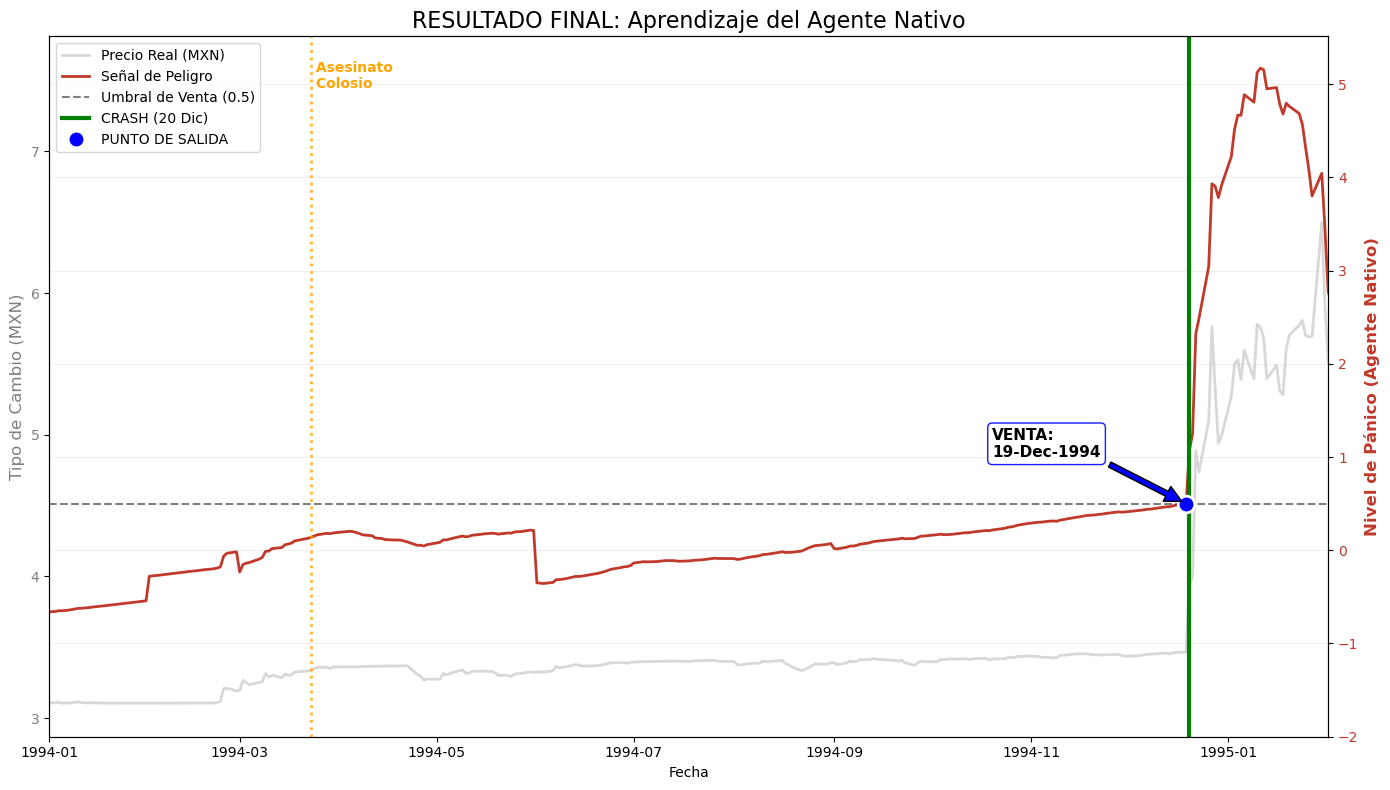
\includegraphics[width=1.0\textwidth]{graf_mexico_final.png}}
    \caption{Predicción México 1994: El agente con pesos UK y umbral calibrado predice correctamente el colapso con 1 día de antelación.}
    \label{fig:mexico_boxed}
\end{figure}
% ----------------------------------------------------------------------------
% 5. CONCLUSION
% ----------------------------------------------------------------------------
\section{Conclusion}

Este trabajo demuestra que la \textit{Danger Theory} ofrece un marco conceptual superior a los modelos econométricos tradicionales para la detección de crisis cambiarias. Nuestras contribuciones principales son:

\begin{enumerate}
    \item \textbf{Hallazgo Empírico:} La intervención del banco central y el desempleo son predictores adelantados infinitamente más confiables que el precio. Un agente artificial puede anticipar crisis con precisión de 1 día.
    \item \textbf{Validación Cruzada:} Los pesos aprendidos en UK generalizan a México tras calibración, validando que la ``física'' subyacente de la crisis es universal.
    \item \textbf{Robustez:} El agente mantiene su comportamiento incluso en escenarios sintéticos radicalmente distintos, descartando overfitting.
    \item \textbf{Metodología Reproducible:} Proporcionamos un pipeline claro (AG para pesos, DE para calibración) que puede aplicarse a otros países y crisis.
\end{enumerate}

\noindent
\textbf{Implicaciones Políticas:} Recomendamos a bancos centrales y reguladores instituir ``Tableros de Control de Peligro'' que monitoricen Índices Compuestos de Estrés Sistémico (intervención + desempleo + volatilidad), en lugar de vigilar únicamente precios nominales. Estos tableros permitirían alertas tempranas y posibilidad de ajustes preventivos.

\textbf{Limitaciones y Futuras Investigaciones:} 
\begin{itemize}
    \item El análisis se limita a dos casos históricos. Más muestras (1970s, crisis asiática 1997) reforzarían las conclusiones.
    \item Asumimos linealidad en la combinación de genes. Técnicas de \textit{Deep Learning} (redes neuronales recurrentes) podrían capturar dinámicas no lineales.
    \item Aplicar a tipos de cambio flotantes requeriría redefine el ``crash'', ya que la devaluación es gradual.
\end{itemize}